Die Hauptfortbewegungsarten in Tübingen sind zu Fuß, per Fahrrad oder dem Bus, da in Tübingen alles nicht weit entfernt ist. Wer sehr sportlich ist kommt mit Fuß und Fahrrad auch zum Sand oder zur Morgenstelle. Da Tübingen jedoch sehr hügelig ist\footnote{\url{https://youtu.be/5xBSrqpiiCk}}, empfiehlt es sich für Normalsterbliche, ein Semesterticket zu erwerben.	%TODO insert \link{}{}?
\vfill \pagebreak
\subsubsection*{Mit dem Bus}
Die günstigste Art die Tübinger Busse zu nutzen ist, sich ein Semesterticket zu kaufen. Man zahlt zu Beginn des Semesters \Ticketpreis (der Rest ist im Sozialbeitrag enthalten, den ihr an das Studentenwerk entrichten müsst).  Damit kann man dann innerhalb des \emph{Naldo-Bereichs}, das sind die Landkreise Tübingen, Reutlingen, Zollern-Alb sowie Sigmaringen (und einzelne Strecken in angrenzenden Landkreisen), alle öffentlichen Verkehrsmittel benutzen. Dazu zählen sowohl die Stadtbusse aller genannten Städte, als auch sämtliche Züge (außer IC) und Regionalbusse, die in dieser Region fahren.

Das Ticket bekommt ihr unter anderem in den Reisezentren in Reutlingen und Tübingen sowie in der Touristeninformation Tübingens an der Neckarbrücke. Zum Kauf müsst ihr euren Studentenausweis und den kleinen Abschnitt "`Bescheinigung für das Semesterticket"' des großen Bescheinigungsbogens mitbringen, der euch nach der Einschreibung per Post zugeschickt wurde.

Seit dem Wintersemester 2014/2015 gilt außerdem die Freizeitregelung von Naldo. Damit könnt ihr unter der Woche ab 19 Uhr und am Wochenende ganztägig Busse und Bahnen innerhalb des Naldo-Gebiets kostenlos nutzen. Dafür braucht ihr einfach nur euren Studentenausweis mit dem Naldo-Logo darauf. Falls ihr also nur abends und/oder am Wochenende auf den Bus angewiesen seid, könnt ihr euch u.U. den Anschaffungspreis für das Semesterticket sparen.
Zusätzlich gilt im Tübingen seit Februar 2018 der \emph{ticketfreie Samstag}. Will heißen: Ihr könnt von Freitag Mitternacht bis Sonntag früh um 5 Uhr alle Busse im Tübinger Stadtgebiet kostenfrei nutzen. Dies ist vor allem praktisch für Freunde und Eltern, die euch in Tübingen besuchen und keinen Studentenausweis mit naldo-Logo besitzen. Kostenfrei sind Samstags ebenfalls die Nachtbusse und die Linien nach Hirschau und Bühl, aber nicht die regionalen Buslinien nach Kusterdingen, Reutlingen oder Mössingen. 

Sehr attraktiv sind auch die Donnerstag- (Clubhaus!), Freitag- und Samstag Nacht bis ca. 4.30 Uhr verkehrende Nachtbusse.  Die Takte sind hier zwar nur (halb-)stündlich und die Fahrt dauert vielleicht etwas länger als normal, aber Mensch kommt sicher Heim (egal, in welchem Zustand).  Also noch ein Grund, das Semesterticket zu erwerben, da es auch für die Nachtbusse gilt. An den anderen Tagen fährt der Nachtbus bis ca. 3 Uhr.

\begin{center}
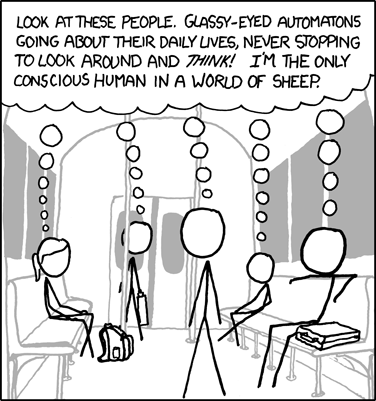
\includegraphics[width=0.5\hsize]{info/xkcd/sheeple.png}
\end{center}

\subsubsection*{Mit dem Fahrrad}
Wie in den meisten Unistädten wird in Tübingen sehr viel Fahrrad gefahren. Es gibt daher auch vor allen wichtigen Gebäuden die Möglichkeit sein Fahrrad anzuschließen. Darüber kann das Fahrrad im Bus die steilen Anstiege mitgenommen werden (zumindest wenn nicht gerade Sperrzeit ist, in vielen Bussen befindet sich dazu ein Aushang).

\subsubsection*{Zu Fuß}
Wie bereits erwähnt sind die meisten Wege in Tübingen sehr kurz, sodass man selten mehr als eine halbe Stunde laufen muss, um sein Ziel zu erreichen. Dies ist vor allem praktisch, wenn das Rad mal wieder einen Platten hat oder man den letzten Bus verpasst hat.

\subsubsection*{Die SAMs}
Ist der Weg doch mal zu weit oder die Füße zu müde gibt es noch die Möglichkeit ein SAM (\textbf{S}ammel\textbf{a}nruf
\textbf{M}ietfahrzeug) zu rufen. Gerade wenn man in einem der ausgelagerten Vororte von Tübingen, wie Hirschau,
Weilheim, Unterjesingen, ..., wohnt ist dies sehr praktisch. Das SAM bringt euch von Haustür evtl. über Umwege zu Haustür (in der Innenstadt nur von/zu bestimmten SAM-Treffpunkten).

\subsubsection*{Mit dem Auto}
Wer trotz dieses guten Angebots an Nahverkehrsmittel mit dem Auto kommen will/muss, sollte folgendes beachten: Kostenlose Parkplätze gibt es nur auf dem Sand, nicht auf der Morgenstelle.  Dort benötigt man für den studentischen Parkplatz eine Nutzungsberechtigung, die man aber nur erhält, wenn die Fahrzeit mit Bus und Bahn länger als 40 Minuten dauern würde (Inwieweit es hier für Informatikstudenten Ausnahmen gibt, ist derzeit unklar), außerdem ist die Anzahl an Parkplätzen sehr begrenzt.

 Erledigen könnt ihr die Freischaltung in dem Büro schräg gegenüber dem Studententerminal im Hörsaalzentrum (direkt neben dem Ausgang Richtung Neubau Chemie). Ihr müsst dafür aber unbedingt das Datenkontrollblatt mitbringen, welches euch per Post zugeschickt wurde. Für alle anderen mit kürzerer Fahrzeit steht oberhalb der Morgenstelle ein kostenpflichtiges Parkhaus zur Verfügung. Wenn ihr eine Parkkarte für das ganze Semester kauft, wird's deutlich günstiger. Infos zu den Tarifen des Parkhauses findet ihr unter \url{https://www.pbw.de/?cmd=Dauerparker&id_city=11&id_object=58}.

\subsubsection*{Von und nach Tübingen}
Wer nach Tübingen oder von Tübingen wegfährt, kann dies gut mit Auto, Bahn oder Fernbus. Züge fahren fast stündlich nach Stuttgart, von wo man dann Fernzüge in alle deutschen Großstädte nehmen kann. Fährt man mit dem Auto, empfiehlt es sich, über die B27 zu fahren. Wer lieber günstig, aber dafür länger fahren will, kann auch einen Fernbus nehmen. Diese fahren mehrmals täglich am Tübinger Hauptbahnhof.
